% $Header: /Users/joseph/Documents/LaTeX/beamer/solutions/generic-talks/generic-ornate-15min-45min.en.tex,v 90e850259b8b 2007/01/28 20:48:30 tantau $

\documentclass[svgnames,smaller]{beamer}

% This file is a solution template for:

% - Giving a talk on some subject.
% - The talk is between 15min and 45min long.
% - Style is ornate.



% Copyright 2004 by Till Tantau <tantau@users.sourceforge.net>.
%
% In principle, this file can be redistributed and/or modified under
% the terms of the GNU Public License, version 2.
%
% However, this file is supposed to be a template to be modified
% for your own needs. For this reason, if you use this file as a
% template and not specifically distribute it as part of a another
% package/program, I grant the extra permission to freely copy and
% modify this file as you see fit and even to delete this copyright
% notice. 

\mode<presentation>
{
  \usetheme{Darmstadt}
 	\usecolortheme[named=ForestGreen]{structure}

  \setbeamercovered{transparent}
  % or whatever (possibly just delete it)
}


\usepackage[english]{babel}
% or whatever

\usepackage[latin1]{inputenc}
% or whatever

\usepackage{times}
\usepackage[T1]{fontenc}
% Or whatever. Note that the encoding and the font should match. If T1
% does not look nice, try deleting the line with the fontenc.

\usepackage{booktabs}
\usepackage{array}
\usepackage{graphicx}
\usepackage{tikz}

\title[Statistical Analysis] % (optional, use only with long paper titles)
{Statistical Analyses on Legacy data of the GRSM Stream Survey}

\subtitle
{Time Trend Analysis, ANOVA, Power Analysis} % (optional)

\author[Pobst, Tim] % (optional, use only with lots of authors)
{Tim Pobst}

\institute[University of Tennesssee Knoxville] % (optional, but mostly needed)
{Department of Civil and Environmental Engineering\\
University of Tennessee}

\date[Thesis Defense] % (optional)
{\today}

\subject{Talks}
% This is only inserted into the PDF information catalog. Can be left
% out. 

\pgfdeclareimage[height=0.5cm]{university-logo}{Figures/utlogo-large.jpg}
\logo{\pgfuseimage{university-logo}}

\pgfdeclareimage[height=\paperheight,width=\paperwidth]{smokies}{Figures/smoky_mountains_sunrise_.jpg}
\usebackgroundtemplate{\tikz\node[opacity=0.3]{\pgfuseimage{smokies}};}

%\setbeamertemplate{background canvas}{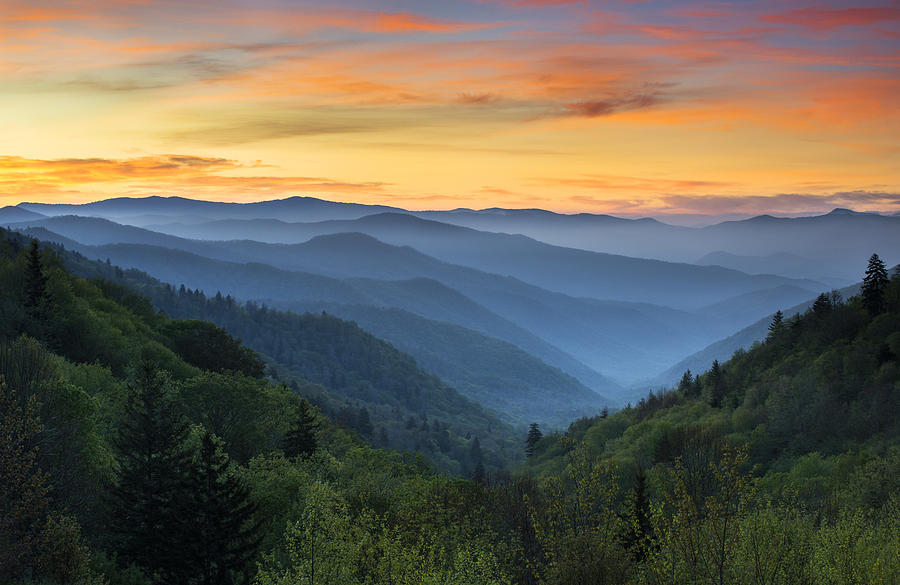
\includegraphics[width=\paperwidth,height =\paperheight]{Figures/smoky_mountains_sunrise_.jpg}}

% If you wish to uncover everything in a step-wise fashion, uncomment
% the following command: 

%\beamerdefaultoverlayspecification{<+->}
%%%%%%%%%%%%%%%%%%%%%%%%%%%%%%%%%%%%%%%%%%%%%%%%%%%%%%%%%%%%%%%%%%%%%%%%%%%%%%%%%%%
%%%%%%%%%%%%%%%%%%%%%%%%%%%%%%%%%%%%%%%%%%%%%%%%%%%%%%%%%%%%%%%%%%%%%%%%%%%%%%%%%%%
%%%%%%%%%%%%%%%%%%%%%%%%%%%%%%%%%%%%%%%%%%%%%%%%%%%%%%%%%%%%%%%%%%%%%%%%%%%%%%%%%%%
\begin{document}

\begin{frame}
  \titlepage
\end{frame}

\begin{frame}{Contents}
  \tableofcontents
  % You might wish to add the option [pausesections]
\end{frame}
%%%%%%%%%%%%%%%%%%%%%%%%%%%%%%%%%%%%%%%%%%%%%%%%%%%%%%%%%%%%%%%%%%%%%%%%%%%%%%%%%%%
%%%%%%%%%%%%%%%%%%%%%%%%%%%%%%%%%%%%%%%%%%%%%%%%%%%%%%%%%%%%%%%%%%%%%%%%%%%%%%%%%%%
\section{Introduction}

	\subsection{Description of study area}
		\begin{frame}{Study area}

\begin{block}{Description of study area}
	\begin{itemize}
		\item Straddles the border of Tennessee and North Carolina
		\item Diverse wildlife, plant life, and fish life.
	\end{itemize}
\end{block}
 
\begin{figure}
\centering			
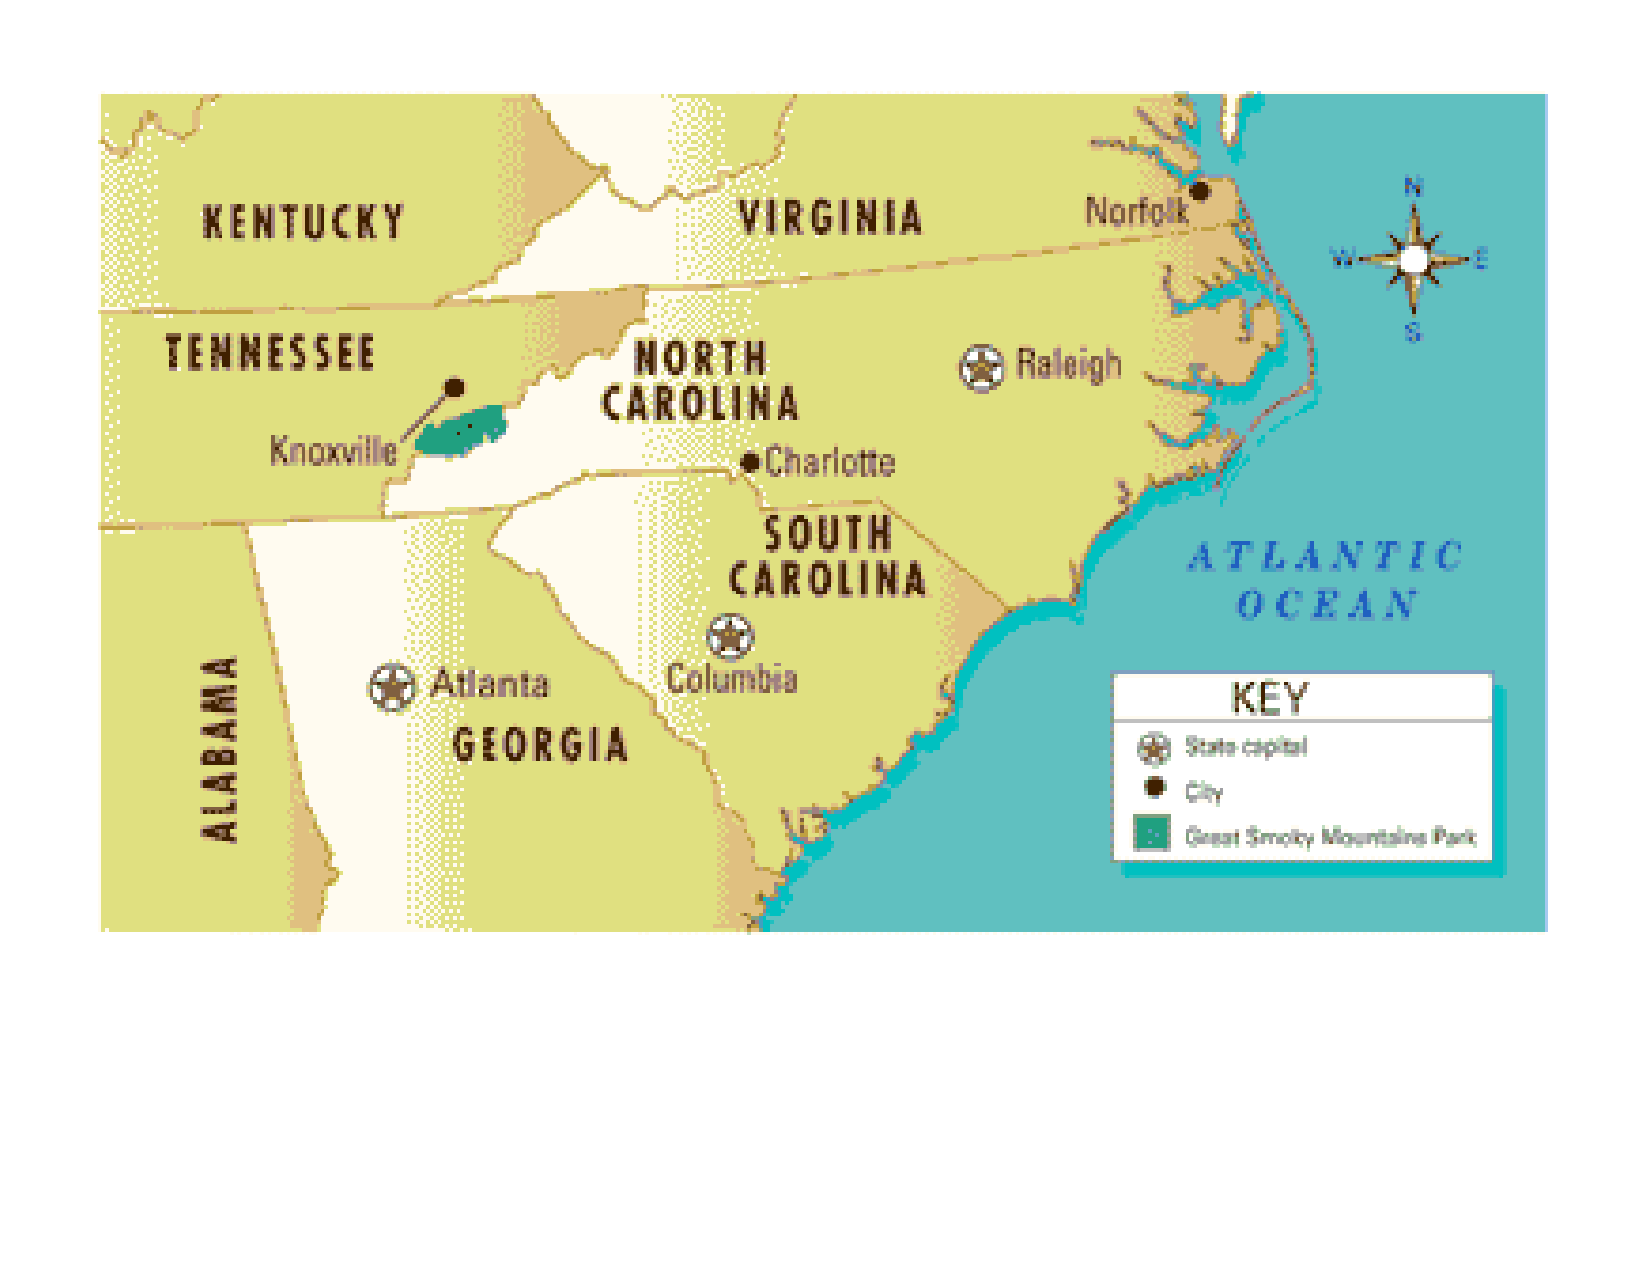
\includegraphics[width=.85\textwidth]{Figures/Parklocation2}
\end{figure}
		
\end{frame}

	\subsection{Acid Deposition and the GRSM}
		\begin{frame}{Acid Deposition and the GRSM}

\begin{block}{Affects and effects}
	\begin{itemize}
		\item Acid deposition negatively affects the park.
		\item Higher elevations are effected worse.
	\end{itemize}
\end{block}
 
\begin{figure}
\centering			
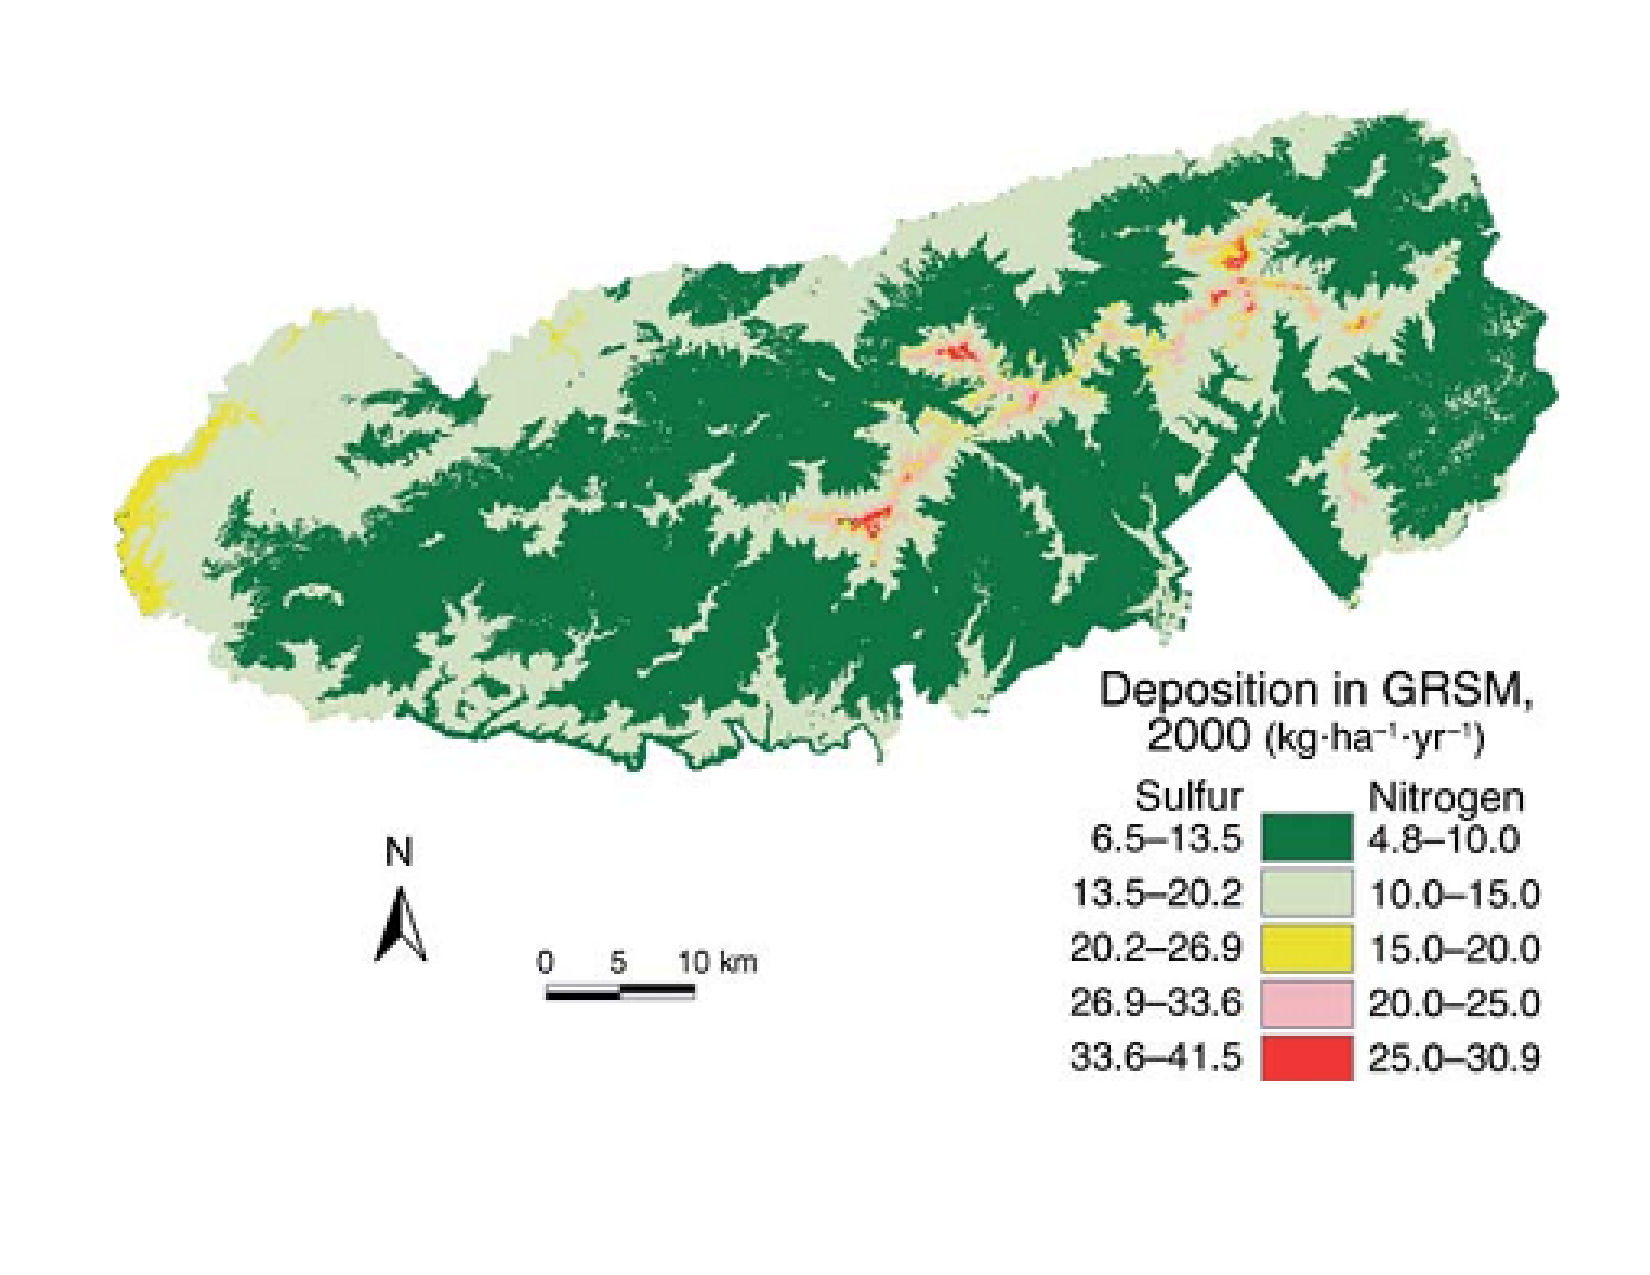
\includegraphics[width=.70\textwidth]{Figures/DepositionHeat}
\end{figure}
		
\end{frame}

	\subsection{Stream Survey}
		\begin{frame}{Database}

\begin{block}{Sites}
	\begin{itemize}
		\item 1993 - ongoing
		\item The number of sites monitored has decreased over the years
	\end{itemize}
\end{block}
 
\begin{figure}
\centering			
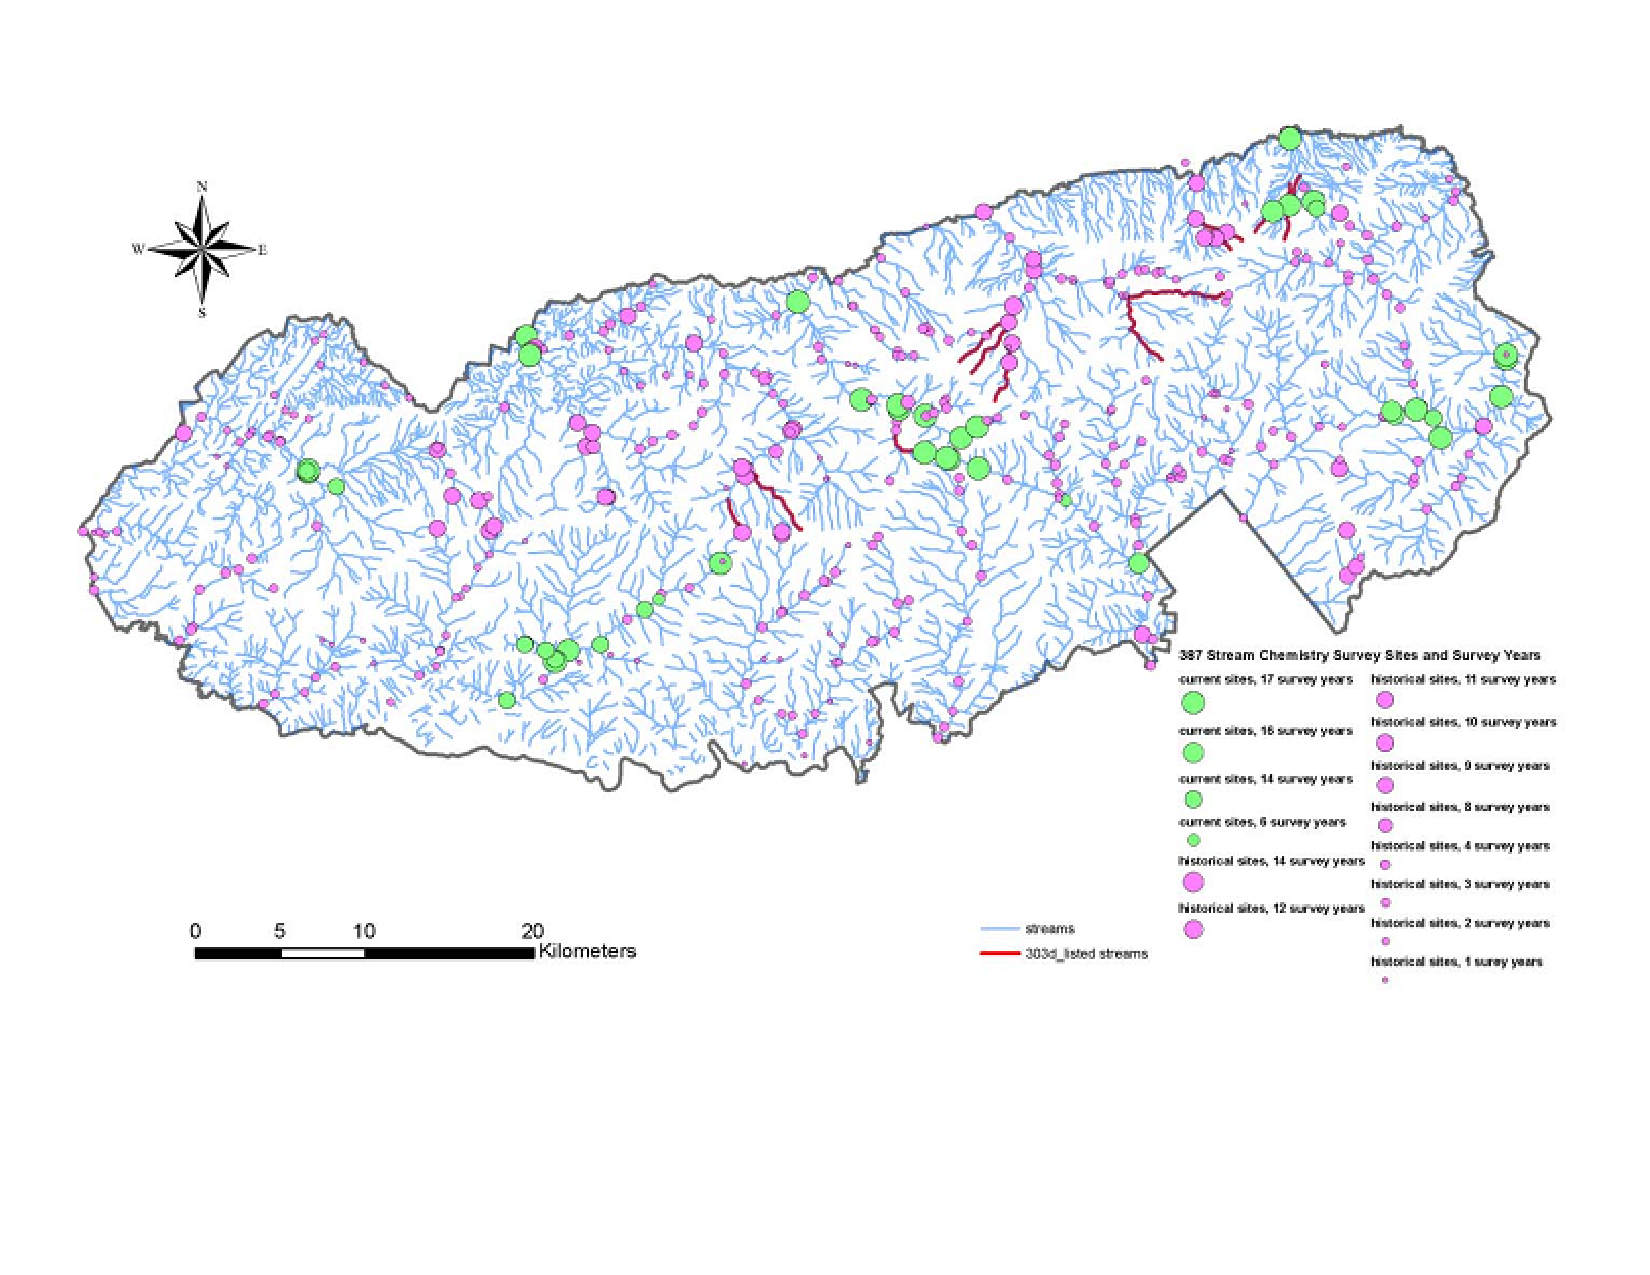
\includegraphics[width=.75\textwidth]{Figures/SSsites}
\end{figure}
		
\end{frame}

		\begin{frame}{Elevation Bands}

\begin{block}{Changes}
	\begin{itemize}
		\item 11 historical elevation bands
		\item re-organized into six	more powerful bands	
	\end{itemize}
\end{block}
			
\begin{table}[h]\footnotesize
%\caption[Proposed elevation classes]{These elevation classes were created to add more weight to the higher elevations.}
\begin{tabular}{p{1.5cm}p{2cm}cp{4.4cm}}
\toprule
Elevation Classes & Meters (Feet)                           & n & Site \# \\ 
\midrule

1                        & 304.8-609.6 (1000-2000)           & 5   & 13 ,23, 24, 30, 479 \\ 
2                        & 609.6-762 (2000-2500)              & 9   & 4, 311, 268, 480, 310, 483, 147, 148, 484 \\ 
3                        & 762-914.4 (2500-3000)              & 13 & 114, 481, 482, 149, 66, 492, 137, 293, 270, 493, 485, 144, 224 \\ 
4                        & 914.4-1066.8 (3000-3500)         & 4   & 143, 142, 73, 71 \\ 
5                        & 1066.8-1371.6 (3500-4500)       & 4   & 74, 221, 251, 233 \\ 
6                        & \multirow{2}{2cm}{$1371.6<$\\$(4500<)$}                    & 2   & 253, 234 \\ 
&&&\\
\bottomrule
\end{tabular}
%\label{tab:ElevationBands}
\end{table}
		
\end{frame}

	\subsection{Time sets}
		\begin{frame}{Time Sets}
	\begin{columns}
	\column{.5\textwidth}
	\begin{block}{3 separate sets}
		\begin{enumerate}
			\uncover<1>{\item \textcolor{blue}{1993-2002:} The years previously studied by Dr. Robinson}
			\uncover<2>{\item \textcolor{blue}{2003-2008:} Up to 2008, the year Kingston and Bull-run installed sulfate scrubbers}
			\uncover<3>{\item \textcolor{blue}{2009-2012:} After the scrubbers were installed up to the most recent data available}
		\end{enumerate}
	\end{block}
	
	\column{.5\textwidth}
	\only<1>{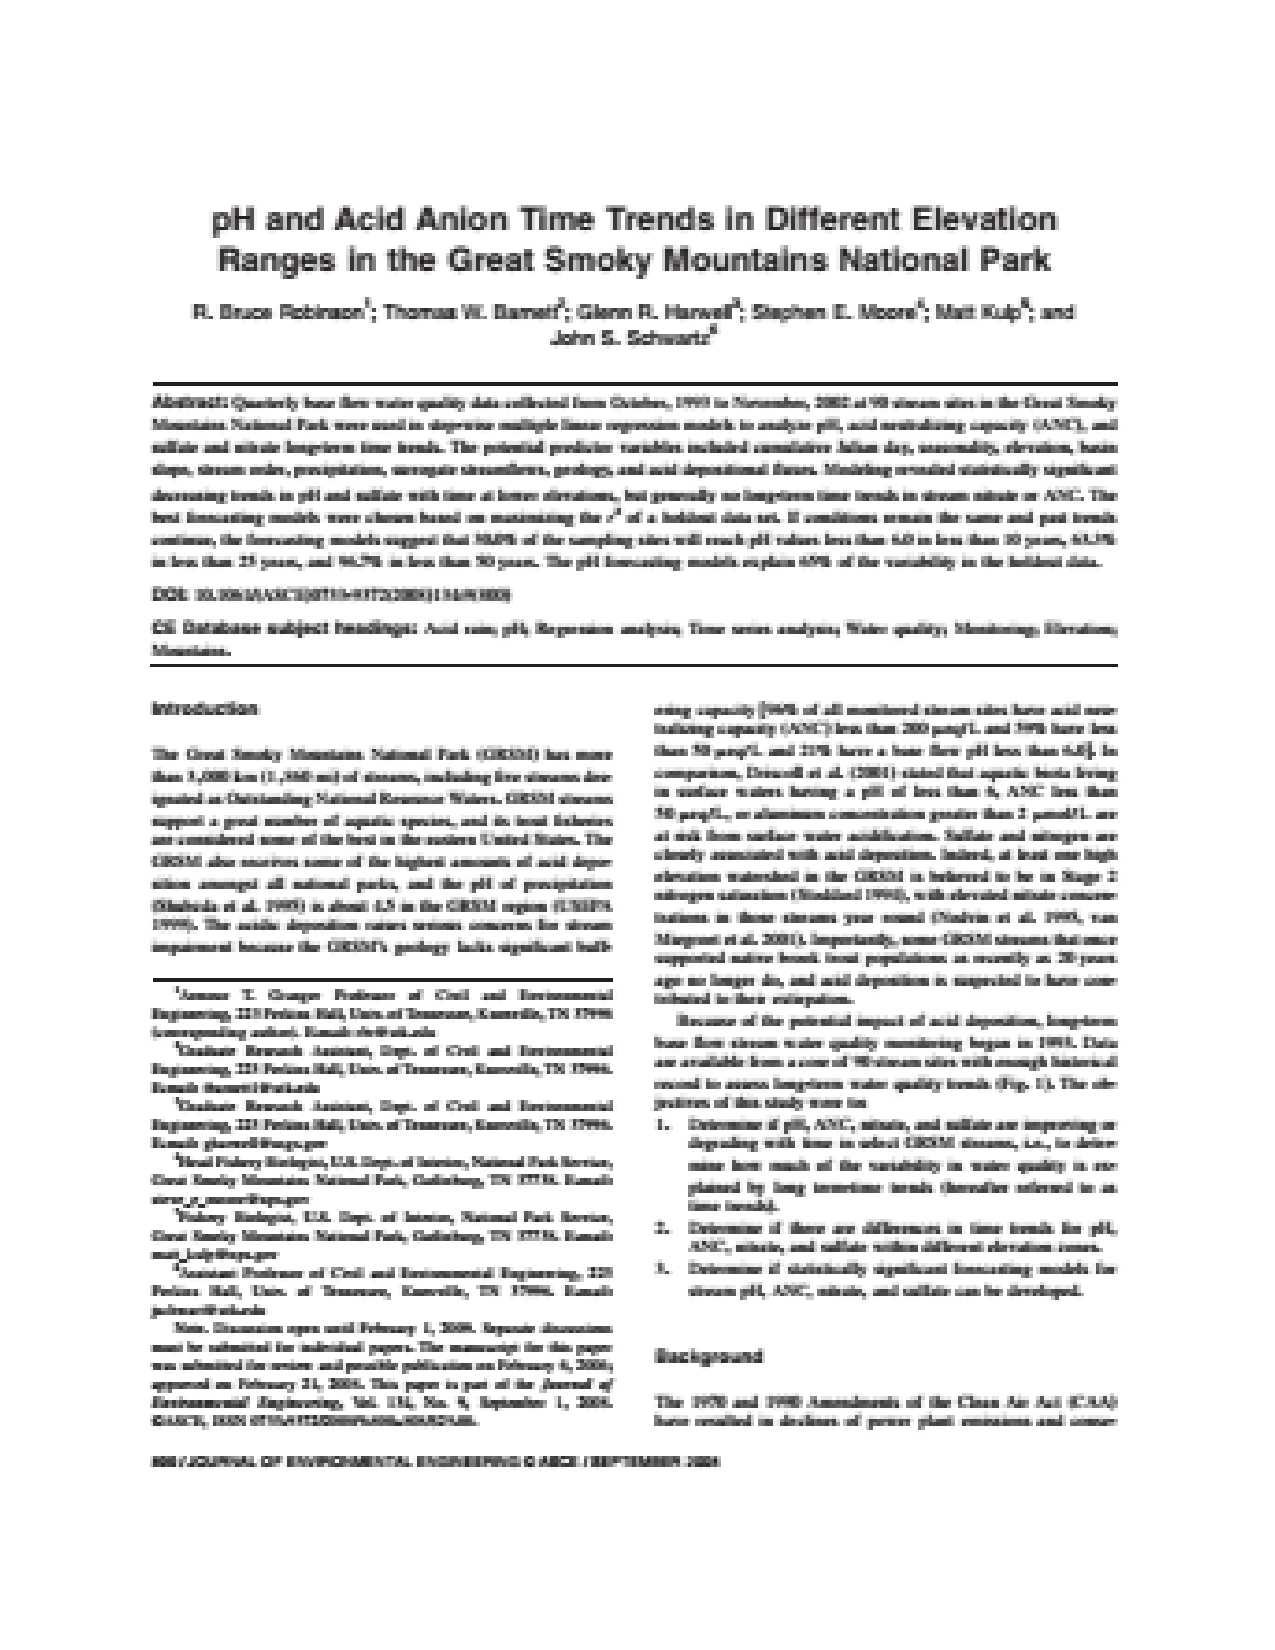
\includegraphics[width=\textwidth]{Figures/Robinson08}}
	\only<2>{\begin{figure}\centering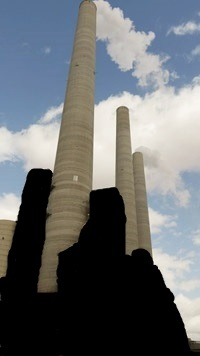
\includegraphics[width=.70\textwidth]{Figures/noscrubber.jpg}\end{figure}}
	\only<3>{\begin{figure}\centering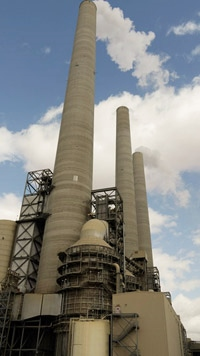
\includegraphics[width=.70\textwidth]{Figures/scrubber.jpg}\end{figure}}
	\end{columns}
\end{frame}
			
	\subsection{Data Smoothing}
		\begin{frame}{Data Smoothing}

\begin{block}{Outliers and Influential observations}
	\begin{itemize}
		\item Influential observations are studied
			\begin{itemize}
				\item Removed Abrams and sites associated with Anakesta
				\item Others are reviewed individually
				\item Outliers remain
			\end{itemize}		
	\end{itemize}
\end{block}
 
\begin{figure}
\centering			
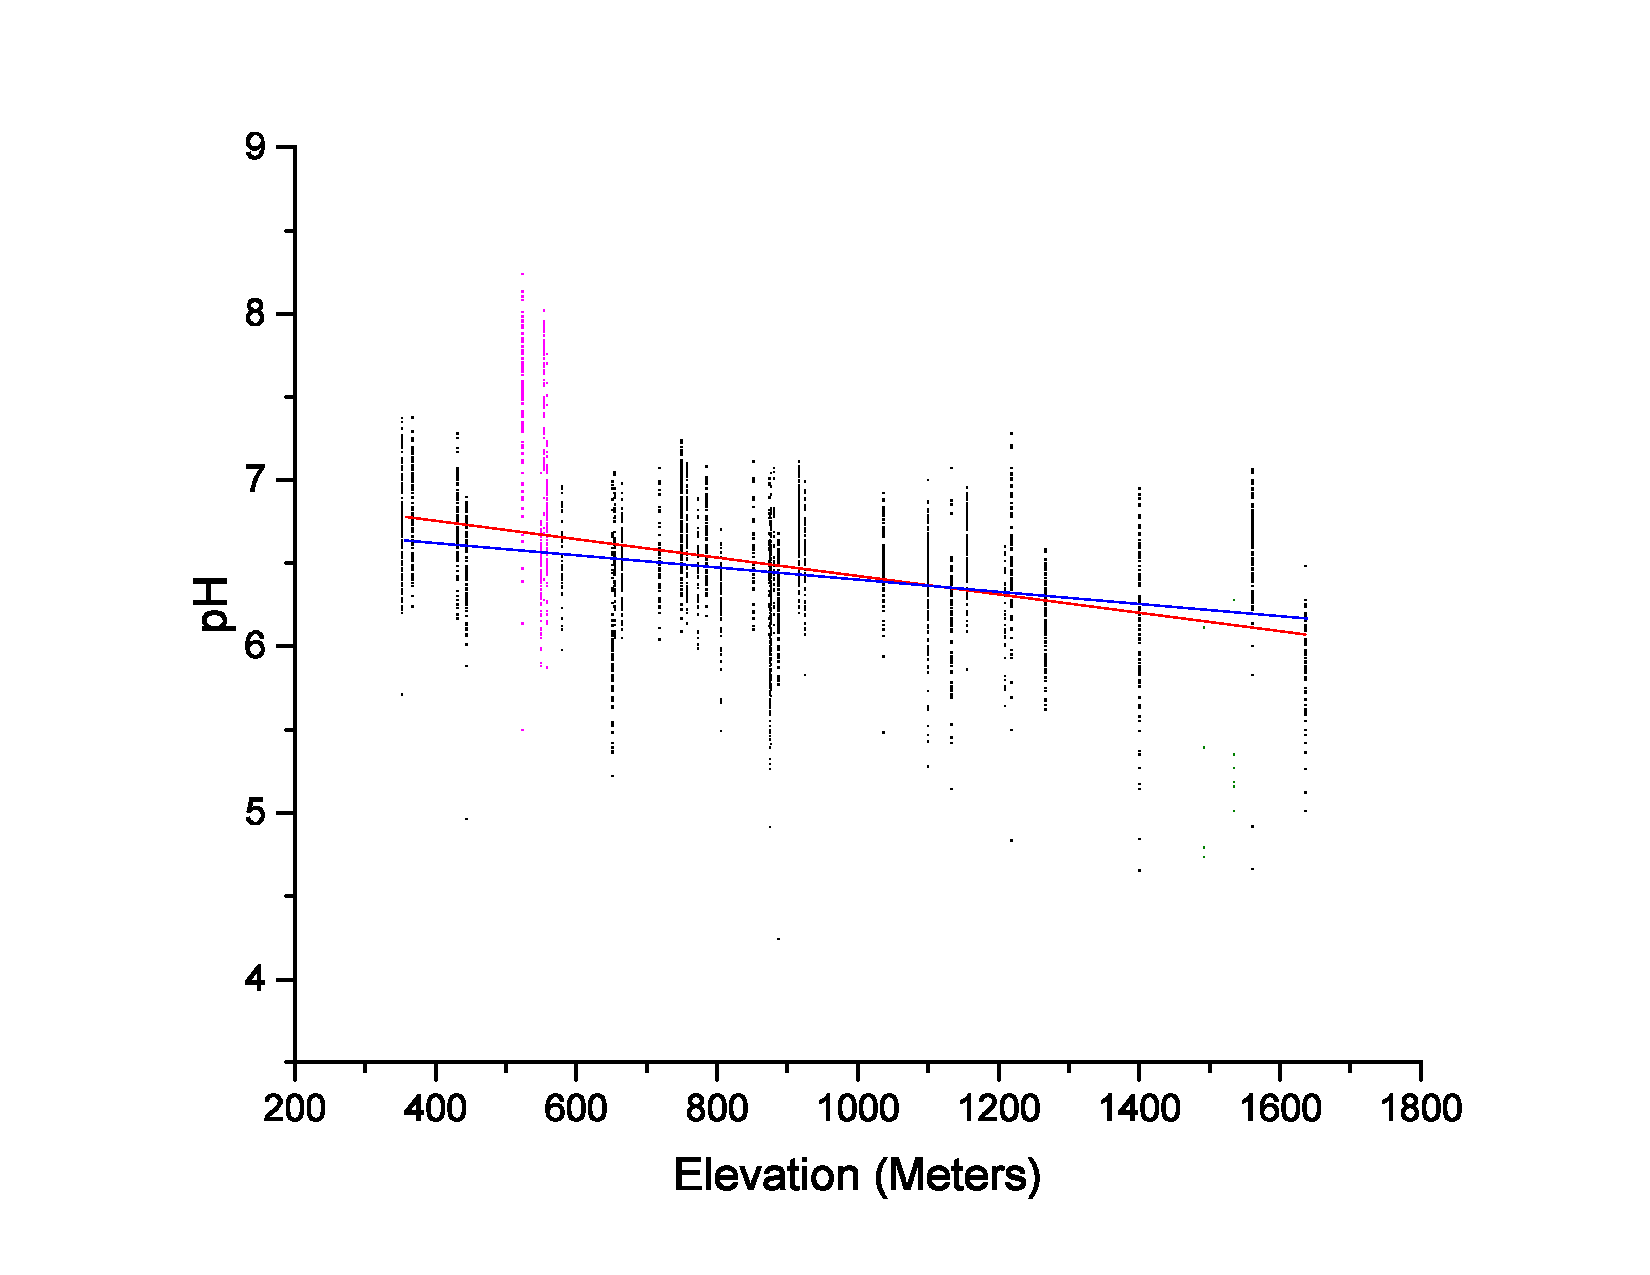
\includegraphics[width=.60\textwidth]{Figures/pHdata}
\end{figure}
		
\end{frame}

	\subsection{Objectives}
		\begin{frame}{Objectives}
	\begin{block}{One}
			 Determine conditions of stream pH and acidic anions within elevation bands.\pause
				\begin{itemize}
					\item Time trends
					\item Means Comparisons
				\end{itemize}\pause
	\end{block}
	\begin{block}{Two}
			Determine statistical power for water quality parameters.\pause
				\begin{itemize}
					\item Post Hoc Analysis
					\item A priori Analysis 
				\end{itemize}		
	\end{block}
\end{frame}

%%%%%%%%%%%%%%%%%%%%%%%%%%%%%%%%%%%%%%%%%%%%%%%%%%%%%%%%%%%%%%%%%%%%%%%%%%%%%%%%%%%
%%%%%%%%%%%%%%%%%%%%%%%%%%%%%%%%%%%%%%%%%%%%%%%%%%%%%%%%%%%%%%%%%%%%%%%%%%%%%%%%%%%
\section{Time Trend Analysis}

	\subsection{Introduction}
		\begin{frame}{Stream Survey trend analysis history}
			\begin{columns}[T]
				\column{.5\textwidth}
					\begin{block}{Robinson 2008}%step-wise equations
						\begin{itemize}
						\uncover<1>{\item Time trends for water quality variables were computed for 90 sites in 10 elevation bands for the years 1993 to 2002.}
						\uncover<2>{\item Predictions for stream pH}
						\end{itemize}		
					\end{block}	
					\begin{block}{Biotics Effects report 2013}
						\begin{itemize}
							\uncover<3>{\item Time trends for water quality variables were computed for 67 sites for the years 1993 to 2009.}
						\end{itemize}		
					\end{block}	
				\column{.5\textwidth}
					\begin{block}{Results}				
						\only<1>{pH is \alert{decreasing} at at rate of -0.0127 to -0.0260 pH units/year for Elevation Classes 2-6.}
						\only<2>{pH will reach a deadly \alert{5.0} in 9.4 years in elevation class 6 (914-1067m)}
						\only<3>{\begin{itemize}
									\item Most showed no trend 
									\item 22 showed an \textcolor{blue}{increase} in pH 
								           \item Only 2 showed a \alert{decrease} 
							       \end{itemize}}
					\end{block}	
						\only<2>{\begin{figure}\centering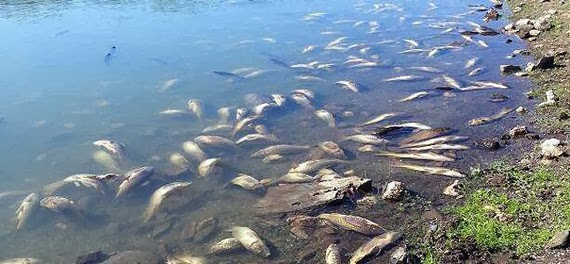
\includegraphics[width=\textwidth]{Figures/spaindeadfish.jpg}\end{figure}}
						\only<3>{\begin{figure}\centering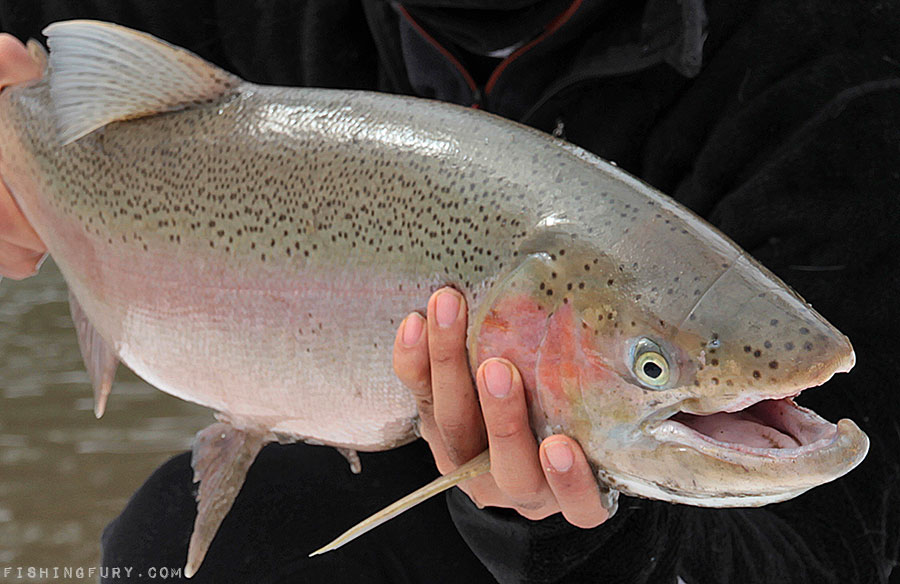
\includegraphics[width=.88\textwidth]{Figures/happy-trout1.jpg}\end{figure}}			
			\end{columns}
\end{frame}
	
	\subsection{Regression}
		\begin{frame}<1-3>{Two equation methods}
	\only<1,3>{\begin{block}{Step-wise: $Y=\beta_0 + \beta_1  T + \beta_2  X + \beta_n X + \epsilon$}
		\begin{itemize}
			\item Multi-step process of adding and removing variables
			\item A variable with an F test statistic of .05 or higher can enter but would be removed if it exceeded .10. %goodness of fit test for the whole equation
			\item If any of the time variables were chosen by the step-wise method, the others were forced in.
		\end{itemize}
	\end{block}}

	\only<2>{\begin{table}[htbp]\scriptsize
\caption[Step-wise equations]{Equations created through step-wise variable selection}
\begin{tabular}{lp{5cm}cc}
\toprule
Dependent (n)     &Model                                                                                                                                                                                                                                                                                                                                                                                                       & Adjusted $r^2$  & Model p \\ 
\midrule
pH (3116)            &$.673\times\log_2(\text{Sum Base Cations}) + (-.368\times \text{NO}_3) + (.262\times \text{Julian Day}) + (-.266\times \text{SO}_4) + (-.050\times\cos(\theta))$                                                                                                                                       & 0.630                  & $<$0.001 \\
ANC (3116)         &$ (.415\times \text{Sum Base Cations}) + (-.185\times \text{SO}_4) + (.595\times \text{Conductivity}) + (-.102\times \text{NO}_3) + (.019\times \text{Julian Date}) + (.005\times \text{Cl}) + (.005\times \sin(\theta))$                                                & 0.984                  & 0.049 \\
NO$_3$ (3116)   &$(-.295\times \text{SO}_4) + (-3.183\times \text{ANC}) + (2.19\times \text{Conductivity}) + ( .923\times \text{Sum Base Cations}) + (.120\times \text{Julian Date}) + (.051\times \text{Cl}) + (.047\times \sin(\theta)) + (.031\times \cos(\theta))$ &0.498                   & 0.017 \\ 
SO$_4$ (3116)   &$ (-.166\times \text{NO}_3) + (2.318\times \text{Conductivity}) + (-3.229\times \text{ANC}) + (1.033\times \text{Sum Base Cations}) + (.042\times \text{Julian Date})$                                                                                                                               & 0.720                  & $<$0.001 \\ 
\bottomrule
\end{tabular}
\label{tab:stepwiseeq}
\end{table}
}

	\only<1,3>{\uncover<3>{\begin{block}{Time Variables: $Y= \beta_0 + \beta_1 Julian Date + \beta_2 \sin(\theta) + \beta_3 \cos(\theta) + \epsilon$}
		\begin{itemize}
			\item Remove the confusion caused by extra non-time based variables
			\item Inherently weaker because time doesn't explain all the variation of the dependent variables.
		\end{itemize}
	\end{block}}}
\end{frame}

		\begin{frame}{Step-wise equations}
	\begin{table}[htbp]\scriptsize
\caption[Step-wise equations]{Equations created through step-wise variable selection}
\begin{tabular}{lp{5cm}cc}
\toprule
Dependent (n)     &Model                                                                                                                                                                                                                                                                                                                                                                                                       & Adjusted $r^2$  & Model p \\ 
\midrule
pH (3116)            &$.673\times\log_2(\text{Sum Base Cations}) + (-.368\times \text{NO}_3) + (.262\times \text{Julian Day}) + (-.266\times \text{SO}_4) + (-.050\times\cos(\theta))$                                                                                                                                       & 0.630                  & $<$0.001 \\
ANC (3116)         &$ (.415\times \text{Sum Base Cations}) + (-.185\times \text{SO}_4) + (.595\times \text{Conductivity}) + (-.102\times \text{NO}_3) + (.019\times \text{Julian Date}) + (.005\times \text{Cl}) + (.005\times \sin(\theta))$                                                & 0.984                  & 0.049 \\
NO$_3$ (3116)   &$(-.295\times \text{SO}_4) + (-3.183\times \text{ANC}) + (2.19\times \text{Conductivity}) + ( .923\times \text{Sum Base Cations}) + (.120\times \text{Julian Date}) + (.051\times \text{Cl}) + (.047\times \sin(\theta)) + (.031\times \cos(\theta))$ &0.498                   & 0.017 \\ 
SO$_4$ (3116)   &$ (-.166\times \text{NO}_3) + (2.318\times \text{Conductivity}) + (-3.229\times \text{ANC}) + (1.033\times \text{Sum Base Cations}) + (.042\times \text{Julian Date})$                                                                                                                               & 0.720                  & $<$0.001 \\ 
\bottomrule
\end{tabular}
\label{tab:stepwiseeq}
\end{table}

\end{frame}%put this in an appendix?

	\subsection{Results}
		\begin{frame}{144 trends analyzed}
			\begin{columns}[T]
				\column{.35\textwidth}
					\begin{block}{Step-wise equations}
						\begin{itemize}[<+->]
							\item pH \uncover<2-8> {\textcolor{blue}{ increasing}}
							\item ANC \uncover<3-8> {\textcolor{blue}{ increasing}}
							\item Nitrate \uncover<4-8> {\alert{increasing}}
							\item Sulfate \uncover<5-8> {\textcolor{blue}{decreasing}}
						\end{itemize}
					\end{block}													
					\begin{block}{Time Variables}
							\uncover<5-8>{Only 20 of the 72 trends are significant}
						\begin{itemize}[<+->]
							\item pH \uncover<6-8> {\textcolor{blue}{ increasing}}
							\item ANC \uncover<7-8> {\textcolor{blue}{ increasing}}
							\item Nitrate
							\item Sulfate
						\end{itemize}
					\end{block}
				\column{.65\textwidth}
					\begin{block}{Trend Results}
						\only<1>{%pH
							      \begin{itemize}
							       	\item pH is \alert{negative} in only 3 significant lines, all in the 93'-02' time set, in elevation classes 2, 3, and 5
								\item Overall pH is \textcolor{blue}{ increasing} over time
							      \end{itemize}
							      }
						\only<2>{%ANC
							      \begin{itemize}
								\item Eleven \textcolor{blue}{positive} trends ranging from\\0.005 to 0.901 $\mu eq L^{-1}$
								\item Seven \alert{negative} trends ranging from\\ -0.002 to -0.082 $\mu eq L^{-1}$
								\item Overall ANC is \textcolor{blue}{ increasing} over time
							       \end{itemize}
							       }
						\only<3>{%Nitrate
							      \begin{itemize}
								\item Trends for time set 1 are half \alert{positive} and half \textcolor{blue}{negative}
								\item Trends in set 2 are all \alert{positive}, from 0.038 to 0.204 $\mu eq L^{-1}$
								\item There is only one \textcolor{blue}{decreasing} trend in set3, class 4 (-0.013 $\mu eq L^{-1}$)
								\item Overall nitrate is \alert{increasing} over time
							       \end{itemize}
							       }
						
						\only<4>{%Sulfate
							      \begin{itemize}
								\item All trends are \alert{positive} in set 2, ranging from 0.034 to 0.161 $\mu eq L^{-1}$
								\item Trends in set 3, classes 1, 3, and 6 are \textcolor{blue}{negative}
								\item Trends are \alert{increasing} from set 1 to set 2, \\ but \textcolor{blue}{decreasing} from set 2 to set 3
							       \end{itemize}
							       }
						\only<5>{%pH
							      \begin{itemize}
							       	\item Set 1 contains 0 significant lines and together sets 2 and 3 are half insignificant
								\item Other than prevalent insignificance, the trends for the time variables are similar to those of the the step-wise equations
								\item Overall pH is slowly \textcolor{blue}{ increasing} over time
							      \end{itemize}
							      }
						\only<6>{%ANC
							      \begin{itemize}
								\item Only 2 of the 24 trends are significant
								\item Set 1, class 5 has a \alert{decreasing} trend\\ of -0.148 $\mu eq L^{-1}$
								\item Set 3, class 5 has a \textcolor{blue}{increasing} trend\\ of 0.891 $\mu eq L^{-1}$
								\item Overall ANC is \textcolor{blue}{ increasing} over time
							      \end{itemize}
							     }
						\only<7>{%Nitrate
							      \begin{itemize}
								\item Only 6 of the 24 trends are significant, 2 in set 1, 4 in set 2, 0 in set 3
								\item Ever trend is \alert{increasing} except set 1, class 1, which is -0.138 $\mu eq L^{-1}$
								\item The increasing trends range from 0.155 $\mu eq/L$ to 0.330 $\mu eq L^{-1}$
								\item Overall nitrate is \alert{increasing} over time
								\item The trends are \textcolor{blue}{decreasing} from set 2 to 3, but all of set 3 is insignificant
							       \end{itemize}
							       }
						\only<8>{%Sulfate
							      \begin{itemize}
								\item Only 5 of the 24 trends are significant, 1 in set 1, 4 in set 2, 0 in set 3
								\item Ever trend is \alert{increasing} except set 1, class 1, which is -0.190 $\mu eq L^{-1}$
								\item The increasing trends range from 0.138 $\mu eq L^{-1}$ to 0.307 $\mu eq L^{-1}$
								\item Overall sulfate is \alert{increasing} over time 
								\item The trends are \textcolor{blue}{decreasing} from set 2 to 3, but all of set 3 is insignificant
							       \end{itemize}
							       }
					\end{block}
			\end{columns}
		\end{frame}
		
		\begin{frame}{Elevation trends}
	\begin{columns}
		\column{.35\textwidth}
			\begin{block}{Three Trends}			
				\begin{itemize}%[<+->]
					\uncover<1>{\item pH and ANC decrease as elevation increases}
					\uncover<2>{\item Nitrate, sulfate, and SBC all increase as elevation increases}
					\uncover<3>{\item Except for SBC all elevational trends decrease over time}
				\end{itemize}
			\end{block}
		\column{.65\textwidth}
			\only<1>{\begin{table}[htbp]\scriptsize
\centering
\caption[Elevation trends]{Dependents regressed against elevation.}
\begin{tabular}{llcccc}
\toprule
set & Dependent & n & slope&$r^2$&per +1000m \\ 
\midrule
1   & pH               & 1357 & .000 & .173 & \textcolor{cyan}{-0.411} \\ 
     & ANC            & 1354 & -.056 & .199 & \textcolor{cyan}{-56.227}  \\ 
     &  NO$_3^-$ & 1161 & .032 & .372 & 32.211  \\ 
     &  SO$_4^{2-}$& 1343 & .037 & .108 & 37.371  \\ 
     & SBC             & 1358 & .013 & .005 & 13.065 \\ 
\midrule
2   & pH               & 997 & .000 & .094 & \textcolor{cyan}{-0.391}  \\ 
     & ANC            & 997 & -.051 & .157 & \textcolor{cyan}{-50.970} \\ 
     &  NO$_3^-$  & 995 & .031 & .307 & 30.677  \\ 
     &  SO$_4^{2-}$ & 1029 & .036 & .098 & 35.793  \\ 
     & SBC             & 1031 & .016 & .009 & 15.537  \\ 
 \midrule
3   & pH              & 757 & .000 & .061 & \textcolor{cyan}{-0.286}  \\ 
     & ANC           & 757 & -.036 & .087 & \textcolor{cyan}{-35.689}  \\ 
     &  NO$_3^-$ & 757 & .026 & .195 & 25.924  \\ 
     &  SO$_4^{2-}$ & 757 & .030 & .101 & 29.715  \\ 
     & SBC            & 757 & .020 & .014 & 19.905  \\ 
 \bottomrule
\end{tabular}
\label{Water quality per elevation}
\end{table}
}
			\only<2>{\begin{table}[htbp]\scriptsize
\centering
\caption[Elevation trends]{Dependents regressed against elevation.}
\begin{tabular}{llcccc}
\toprule
set & Dependent & n & slope&$r^2$&per +1000m \\ 
\midrule
1   & pH               & 1357 & .000 & .173 & -0.411 \\ 
     & ANC            & 1354 & -.056 & .199 & -56.227  \\ 
     &  NO$_3^-$ & 1161 & .032 & .372 & \textcolor{cyan}{32.211}  \\ 
     &  SO$_4^{2-}$& 1343 & .037 & .108 & \textcolor{cyan}{37.371}  \\ 
     & SBC             & 1358 & .013 & .005 & \textcolor{cyan}{13.065} \\ 
\midrule
2   & pH               & 997 & .000 & .094 & -0.391  \\ 
     & ANC            & 997 & -.051 & .157 & -50.970 \\ 
     &  NO$_3^-$  & 995 & .031 & .307 & \textcolor{cyan}{30.677}  \\ 
     &  SO$_4^{2-}$ & 1029 & .036 & .098 & \textcolor{cyan}{35.793}  \\ 
     & SBC             & 1031 & .016 & .009 & \textcolor{cyan}{15.537} \\ 
 \midrule
3   & pH              & 757 & .000 & .061 & -0.286  \\ 
     & ANC           & 757 & -.036 & .087 & -35.689  \\ 
     &  NO$_3^-$ & 757 & .026 & .195 & \textcolor{cyan}{25.924}  \\ 
     &  SO$_4^{2-}$ & 757 & .030 & .101 & \textcolor{cyan}{29.715}  \\ 
     & SBC            & 757 & .020 & .014 & \textcolor{cyan}{19.905}  \\ 
 \bottomrule
\end{tabular}
\label{Water quality per elevation}
\end{table}
}
			\only<3>{\begin{table}[htbp]\scriptsize
\centering
\caption[Elevation trends]{Dependents regressed against elevation.}
\begin{tabular}{llcccc}
\toprule
set & Dependent & n & slope&$r^2$&per +1000m \\ 
\midrule
1   & pH               & 1357 & .000 & .173 & \textcolor{cyan}{-0.411} \\ 
     & ANC            & 1354 & -.056 & .199 & \textcolor{cyan}{-56.227}  \\ 
     &  NO$_3^-$ & 1161 & .032 & .372 & \textcolor{cyan}{32.211}  \\ 
     &  SO$_4^{2-}$& 1343 & .037 & .108 & \textcolor{cyan}{37.371}  \\ 
     & SBC             & 1358 & .013 & .005 & \textcolor{red}{13.065} \\ 
\midrule
2   & pH               & 997 & .000 & .094 & \textcolor{cyan}{-0.391}  \\ 
     & ANC            & 997 & -.051 & .157 & \textcolor{cyan}{-50.970} \\ 
     &  NO$_3^-$  & 995 & .031 & .307 & \textcolor{cyan}{30.677}  \\ 
     &  SO$_4^{2-}$ & 1029 & .036 & .098 & \textcolor{cyan}{35.793}  \\ 
     & SBC             & 1031 & .016 & .009 & \textcolor{red}{15.537}  \\ 
 \midrule
3   & pH              & 757 & .000 & .061 & \textcolor{cyan}{-0.286}  \\ 
     & ANC           & 757 & -.036 & .087 & \textcolor{cyan}{-35.689}  \\ 
     &  NO$_3^-$ & 757 & .026 & .195 & \textcolor{cyan}{25.924}  \\ 
     &  SO$_4^{2-}$ & 757 & .030 & .101 & \textcolor{cyan}{29.715}  \\ 
     & SBC            & 757 & .020 & .014 & \textcolor{red}{19.905}  \\ 
 \bottomrule
\end{tabular}
\label{Water quality per elevation}
\end{table}
}
		\end{columns}
\end{frame}	

		\begin{frame}{Data differences}
			\begin{columns}[T]
			\column{.33\textwidth}
				\begin{block}{Robinson 08}
					\begin{itemize}
						\item 90 sites
						\item 11 elevation classes		
						\item 1993 - 2002,\\ 10 years
						\item includes Abrams and sites 237 and 252
					\end{itemize}
				\end{block}
			\column{.33\textwidth}
				\begin{block}{Schwartz 13}
					\begin{itemize}
						\item 67 sites
						\item 11 elevation classes
						\item 1993 - 2009,\\ 17 years
					\end{itemize}
				\end{block}
			\column{.33\textwidth}
				\begin{block}{Pobst 14}
					\begin{itemize}
						\item 43 sites
						\item 6 elevation classes						
						\item set 1: 10 years
						\item set 2: 6 years
						\item set 3: 4 years
						\item removed Abrams and sites 237 and 252
					\end{itemize}
				\end{block}
			\end{columns}
		\end{frame}

		\begin{frame}{Elevation Trend Results by comparison}
	\begin{columns}[T]
		\column{.33\textwidth}
			\begin{block}{Robinson 08}
				\begin{itemize}
					\uncover<1>{\item pH decreases -0.72 pH units \\per 1000 m gain}
					\uncover<2>{\item Elevation not a predictor for any other dependent}
				\end{itemize}
			\end{block}
		\column{.33\textwidth}
			\begin{block}{Schwartz 13}
				\begin{itemize}
					\uncover<1>{\item pH decreases -1.056 pH units per 1000 m gain}
					\uncover<2>{\item ANC decreases -117.909 $\mu eq L^{-1}$ per 1000 m gain}
					\uncover<3>{\item Insignificant negative trend for sulfate}
				\end{itemize}
			\end{block}
		\column{.33\textwidth}
			\begin{block}{Pobst 14}
				\begin{itemize}
					\uncover<1>{\item pH decreases -0.0286 pH units per 1000 m gain}
					\uncover<2>{\item ANC decreases -35.689 $\mu eq L^{-1}$ per 1000 m gain}
					\uncover<3>{\item Positive sulfate elevational trends decrease over time}
					%\item SBC elevational trends increase over time\\ first by 2 $\mu eq L^{-1}$ between sets 1 and 2 \\ then by 5 $\mu eq L^{-1}$ between 2 and 3
				\end{itemize}
			\end{block}
	\end{columns}
\end{frame}	

	\subsection{Discussion and Conclusions}
\begin{frame}
	%\begin{block}{Copnclusions on elevation and time}
		%\begin{itemize}
			%\item elevation was not chosen through the step-wise process
			%\begin{itemize}	
				%\item elevation not as important as other variables
				%\item elevation classes already classify elevation
				%\item elevation classes may be to small for elevation to be important
			%\end{itemize}
			%\item Time may not explain enough variance to use regression for time trends
			%\item agree with the biotics effects report that pH is increasing over time
			%\item sulfate has more decreasing trends for set 3 than any other time set
		%\end{itemize}
	%\end{block}
	\begin{block}{Conclusions on Sulfate}
		sulfate desorption is of greater concern than pH levels in the park
		\begin{itemize}
			\item Lack of trend found in the Biotics effects report were attributed to high elevation soil adsorption of depsotional sulfate
				%sulfate pollution is held between deposition and the streams
			\item Sulfate will remain absorbed to soil particles as long as soil water chemistry remains high in sulfate concentration and low in pH
				%when pH rises and sulfate concentration lowers the extra "held" sulfate pollution will make its way into the streams
			%\item sulfate elevation trends are decreasing overtime but mean concentrations are increasing through time
			\item Over time most sulfate concentrations are positive but in set 3: classes 1, 4, and 6 have negative trends
			\item The elevation trend is decreasing over time
			\item The combination of these trends support desorption of sulfate into the streams bringing the elevation trend to equilibrium
		\end{itemize}
	\end{block}
\end{frame}
		
		
		
%%%%%%%%%%%%%%%%%%%%%%%%%%%%%%%%%%%%%%%%%%%%%%%%%%%%%%%%%%%%%%%%%%%%%%%%%%%%%%%%%%%
%%%%%%%%%%%%%%%%%%%%%%%%%%%%%%%%%%%%%%%%%%%%%%%%%%%%%%%%%%%%%%%%%%%%%%%%%%%%%%%%%%%
\section{ANOVA}

\begin{frame}
	\begin{itemize}\pause
		\item ANOVA/Bonferroni\pause
		\item Discussion
	\end{itemize}
\end{frame}
%%%%%%%%%%%%%%%%%%%%%%%%%%%%%%%%%%%%%%%%%%%%%%%%%%%%%%%%%%%%%%%%%%%%%%%%%%%%%%%%%%%
%%%%%%%%%%%%%%%%%%%%%%%%%%%%%%%%%%%%%%%%%%%%%%%%%%%%%%%%%%%%%%%%%%%%%%%%%%%%%%%%%%%
\section{Power Analysis}

\begin{frame}
	\begin{itemize}\pause
		\item Power Analysis\pause
		\item Post Hoc\pause
		\item A priori\pause
		\item Manipulation
	\end{itemize}
\end{frame}
%%%%%%%%%%%%%%%%%%%%%%%%%%%%%%%%%%%%%%%%%%%%%%%%%%%%%%%%%%%%%%%%%%%%%%%%%%%%%%%%%%%
%%%%%%%%%%%%%%%%%%%%%%%%%%%%%%%%%%%%%%%%%%%%%%%%%%%%%%%%%%%%%%%%%%%%%%%%%%%%%%%%%%%
\section*{Summary}

\begin{frame}{Summary}

  % Keep the summary *very short*.
  \begin{itemize}
  \item
    \alert{Water Quality is getting better}\pause
  \item
    \alert{Sulfate sequestration is supported}\pause
  \item
    \alert{The power of the time trends are excelent}\pause
  \item
     \alert{Power analysis can help re-distribute sites}\pause
  \end{itemize}
  
  % The following outlook is optional.
  \vskip0pt plus.5fill
  \begin{itemize}
  \item
    Outlook
    \begin{itemize}
    \item
     Elevation Bands
    \item
      Effects of sulfate scrubbers
    \end{itemize}
  \end{itemize}
\end{frame}
%%%%%%%%%%%%%%%%%%%%%%%%%%%%%%%%%%%%%%%%%%%%%%%%%%%%%%%%%%%%%%%%%%%%%%%%%%%%%%%%%%%
%%%%%%%%%%%%%%%%%%%%%%%%%%%%%%%%%%%%%%%%%%%%%%%%%%%%%%%%%%%%%%%%%%%%%%%%%%%%%%%%%%%

\end{document}


